\chapter{Generating Fractals using Geometric Algebra}

Fractals have always been a popular topic in computer graphics due
to their ability to give rise to great aesthetic beauty from a relatively
simple mathematical description. Generally a fractal is considered to be
any geometric object which posesses detail on all scales\cite{FRAC:FractalsEverywhere,
  FRAC:FractalGeometryOfNature}. That is to say
that one may examine the edge of the object under arbitrary magnification
yet still find it rough and irregular. Many introductions to the 
subject of fractals and their creation on computers exist\cite{FRAC:FractalGeometry, FRAC:ChaosAndFractals, FRAC:FractalImages}.

The term fractal was coined by Mandelbrot\cite{FRAC:LesObjetsFractals} in 1975,
originally from the latin {\em fractus} (broken). In this chapter we
investigate an extension into GA of the class of fractals he is most 
associated with which are based on repeated iteration of a complex function.
Fractals have found applications in a wide selection of research areas
including image compression (FIXME Citation) and it is supected that the 
GA-based approach here may also be of use in a similar manner.

\section{Fractals from Complex Iteration}

\begin{figure}
\centering
\begin{tabular}{c@{$\quad$}c}
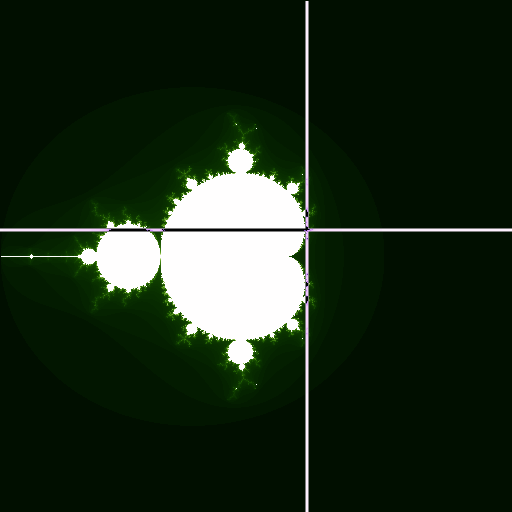
\includegraphics[width=0.4\textwidth]{euc_mandel_julia_pos} 
 & 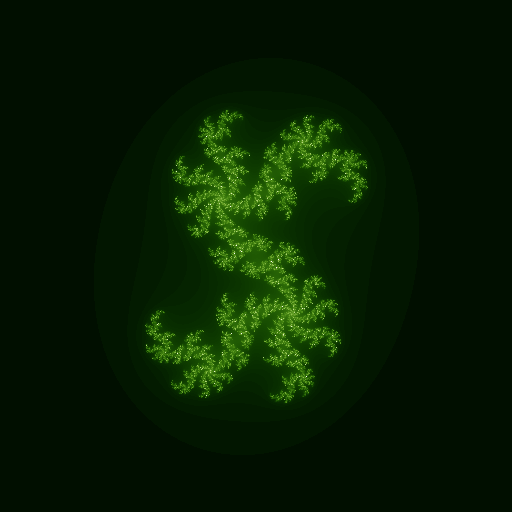
\includegraphics[width=0.4\textwidth]{julia_euc} \\
                          (a) & (b)
\end{tabular}
\caption{\label{fig:euclidean_sets}The well known (a) Mandelbrot set with
  the constant $c = 0.4 + 0.2i$ marked and (b) the Julia
  set associated with $c$.}
\end{figure}

The well-known Mandelbrot and Julia sets (figure \ref{fig:euclidean_sets}) 

We shall examine a common form of fractals generated by the iteration
of some complex function. The well-known 
Mandelbrot
and Julia sets\cite{FRAC:Mandelbrot, FRAC:JuliaMandelBook} are all
generated using the following complex recurrence relation:
\begin{definition}
The complex function $z(n,c)$ is defined as
\[
z(n,c) = z^2(n-1,c) + c
\]
with initial values being defined by a particular fractal.
\end{definition}

\subsection{The Mandelbrot Set}

\begin{definition}[The Mandelbrot set]
The Mandelbrot set, $\mathbb{M}$, is defined as
\[
\mathbb{M} = 
\left\{x \in \mathbb{C} 
: \lim_{n \rightarrow \infty} \magof{z(n,x)} < \infty \right\} 
\]
where $\magof{\cdot}$ is the usual Euclidean $2$-norm and $z(0,c) = 0$.
\end{definition}

\subsection{The Julia Set}

There are an infinite number of Julia sets, each associated with
a particular point on the complex plane. 

\begin{definition}[The Julia set]
The Julia set associated
with the complex number $c$, $\mathbb{J}_c$, is given by
\[
\mathbb{J}_c = 
\left\{x \in \mathbb{C}
: \lim_{n \rightarrow \infty} \magof{z(n,c)} < \infty \right\} 
\]
where $z(0,c) = x$.
\end{definition}

\section{Extending Complex Numbers}

In this section we will seek to find a geometric, co-ordinate free
analogue to the complex mapping $z \mapsto z^2$. We will start by 
confining ourselves to the complex plane and then move into higher dimensions.

Firstly, we need a mapping between the complex numbers, $\mathbb{C}$, and
the vectors in the complex plane, $\mathbb{R}^2$. Letting $\{e_1, e_2\}$
be some orthonormal basis for $\mathbb{R}^2$ we can form a natural
one-to-one mapping between $z \in \mathbb{R}^2$ and $C(z) \in \mathbb{C}$:

\begin{definition}
Given some vector $z \in \mathbb{R}^2$, we can map one-to-one into the
complex plane by forming the complex number
\[
C(z) = (z \cdot e_1) + (z \cdot e_2)i.
\]
\end{definition}

Here it is clear that $e_1$ corresponds to the real-axis and $e_2$ 
corresponds to the imaginary axis of the complex plane.
It is now trivial to show that
\begin{align*}
C^2(z) &= [(z \cdot e_1) + (z \cdot e_2)i]^2 \\
       &= (z \cdot e_1)^2 - (z \cdot e_2)^2 + 2(z \cdot e_1)(z \cdot e_2)i.
\end{align*}

We seek some mapping $z \mapsto z'$ such that $C(z') = C^2(z)$. It is 
easy to verify by direct substitution that the mapping 
$z \mapsto ze_1$ satisfies this and hence is a geometric analogue of 
squaring a complex number:

\begin{lemma}
Given some vector $z \in \mathbb{R}^2$ representing the complex number
$C(z)$, the mapping $z \mapsto ze_1$ is equivalent to $C(z) \mapsto C^2(z)$.
\end{lemma}
\begin{proof}
Let $z = xe_1 + ye_2$. Therefore $C(z) = x + yi$. It is clear that
\begin{align*}
ze_1z &= (x^2 - y^2) e_1 + 2xye_2 \\
\Rightarrow\;C(ze_1z) &= (x^2 - y^2) + 2xyi\\
        &= C^2(z)
\end{align*}
as required.
\end{proof}

To complete the extension one must also define a geometric equivalent of
addition:
\begin{lemma}
Given vectors $z, c \in \mathbb{R}^2$ representing the complex numbers
$C(z)$ and $C(c)$, the mapping $z \mapsto z + c$ is equivalent to 
$C(z) \mapsto C(z) + C(z)$.
\end{lemma}
\begin{proof}
Clear by direct substitution.
\end{proof}

\section{Moving to Higher Dimensions}

We now form an analogy to complex numbers in higher dimensions
by removing the constraint that the vectors need be in $\mathbb{R}^2$.

\begin{definition}
Given a vector $z$ and some unit basis vector $e_1$ the mapping
$z \mapsto ze_1z$ is the geometric analogue of squaring a complex number.
\end{definition}

\begin{definition}
Given two vectors, $z$ and $c$, the geometric analogue of complex addition
is $z \mapsto z + c$.
\end{definition}

We may now define generalised Mandelbrot and Julia sets based upon
a new vector recurrence relation
\begin{definition}
The vector analogue of $z(n,c)$ is defined as
\[
z_v(n,c) = z_v(n-1,c) e_1 z(n-1,c) + c
\]
with initial values being defined by a particular fractal.
\end{definition}

\subsection{The Generalised Mandelbrot Set}

\begin{definition}[The generalised Mandelbrot set]
The generalised Mandelbrot set, $\mathbb{M}_k$, in $\mathbb{R}^k$ 
    is defined as
\[
\mathbb{M}_k = 
\left\{x \in \mathbb{R}^k 
: \lim_{n \rightarrow \infty} z_v^2(n,x) < \infty \right\} 
\]
where $z(0,c) = 0$.
\end{definition}

\subsection{The Generalised Julia Set}

\begin{definition}[The generalised Julia set]
The generalised Julia set, $\mathbb{J}_{c,k}$, in $\mathbb{R}^k$
which is associated with the vector $c \in \mathbb{R}^k$ is given by
\[
\mathbb{J}_{c,k} = 
\left\{x \in \mathbb{R}^k
: \lim_{n \rightarrow \infty} z_v^2(n,c) < \infty \right\} 
\]
where $z(0,c) = x$.
\end{definition}

\subsection{Ray Tracing}

\section{Moving to Hyperbolic Geometry}

\subsection{The Hyperbolic Mandelbrot Set}

\subsection{The Hyperbolic Julia Set}
